\documentclass[aspectratio=169,11pt]{beamer}
\usepackage[T1]{fontenc}
\usepackage{lmodern,amsmath,amssymb,mathtools,bm,booktabs,array,graphicx,tikz}
\usetikzlibrary{arrows.meta,positioning,calc,decorations.pathreplacing,patterns}
\definecolor{ink}{HTML}{17344D}\definecolor{accent}{HTML}{087E8B}\definecolor{pale}{HTML}{EDF5F5}\definecolor{gold}{HTML}{AD6B19}
\providecommand{\dd}{\,\mathrm{d}}\providecommand{\R}{\mathbb{R}}
\providecommand{\E}{\mathbb{E}}\providecommand{\Var}{\operatorname{Var}}
\providecommand{\Cov}{\operatorname{Cov}}\providecommand{\diag}{\operatorname{diag}}
\providecommand{\norm}[1]{\left\lVert#1\right\rVert}
\providecommand{\abs}[1]{\left|#1\right|}
\usefonttheme{professionalfonts}
\setbeamercolor{normal text}{fg=black,bg=white}
\setbeamercolor{frametitle}{fg=ink,bg=white}
\setbeamercolor{title}{fg=ink}\setbeamercolor{structure}{fg=accent}
\setbeamercolor{block title}{fg=ink,bg=pale}\setbeamercolor{block body}{fg=black,bg=pale!40}
\setbeamercolor{alerted text}{fg=accent}
\setbeamerfont{frametitle}{size=\Large,series=\bfseries}
\setbeamerfont{title}{size=\LARGE,series=\bfseries}
\setbeamertemplate{navigation symbols}{}
\setbeamersize{text margin left=.7cm,text margin right=.7cm}
\setbeamertemplate{frametitle}{\vspace{.18cm}\insertframetitle\par\vspace{.1cm}{\color{accent}\hrule height .6pt}\vspace{.12cm}}
\newcommand{\notestarget}{notes.pdf}\newcommand{\noteslabel}{Notes}
\setbeamertemplate{footline}{\hspace{.7cm}\color{ink}\scriptsize Computational Cardiology\quad\href{\notestarget}{\noteslabel}\hfill\insertframenumber\,/\,\inserttotalframenumber\hspace{.7cm}\vspace{.18cm}}
\setbeamercovered{invisible}
\hypersetup{pdfauthor={Zan Ahmad},pdftitle={Membrane current balance and voltage-dependent gates},pdfpagemode=UseNone}
\begin{document}
\begin{frame}[plain]\vfill
{\small\color{accent} Computational Cardiology \quad Lecture 9}\par\medskip
{\raggedright\hyphenpenalty=10000\exhyphenpenalty=10000\LARGE\bfseries\color{ink} Membrane current balance and voltage-dependent gates}\par\bigskip
Zan Ahmad\par\smallskip
{\small Fall 2024}\par\vfill\end{frame}
\renewcommand{\notestarget}{notes.pdf\#note-charge-balance-signs-and-current-densities}
\begin{frame}[t,fragile,label=slide-membrane-charge-balance]{Membrane charge balance}
\[C\dot V=I_{\rm stim}-\sum_jg_j(V-E_j).\]\pause{} Outward ionic current is positive; applied inward current is positive.
\end{frame}
\renewcommand{\notestarget}{notes.pdf\#note-charge-balance-signs-and-current-densities}
\begin{frame}[t,fragile,label=slide-densities-and-total-current]{Densities and total current}
\[I_{\rm density}=I_{\rm total}/A.\]\pause{}\[(\mu\mathrm F/\mathrm{cm}^2)(\mathrm{mV}/\mathrm{ms})=\mu\mathrm A/\mathrm{cm}^2.\]
\end{frame}
\renewcommand{\notestarget}{notes.pdf\#note-conductances-and-gate-relaxation}
\begin{frame}[label=slide-voltage-driving-forces-and-conductances-panel-1]{Equal-duration neuronal pulses}
\centering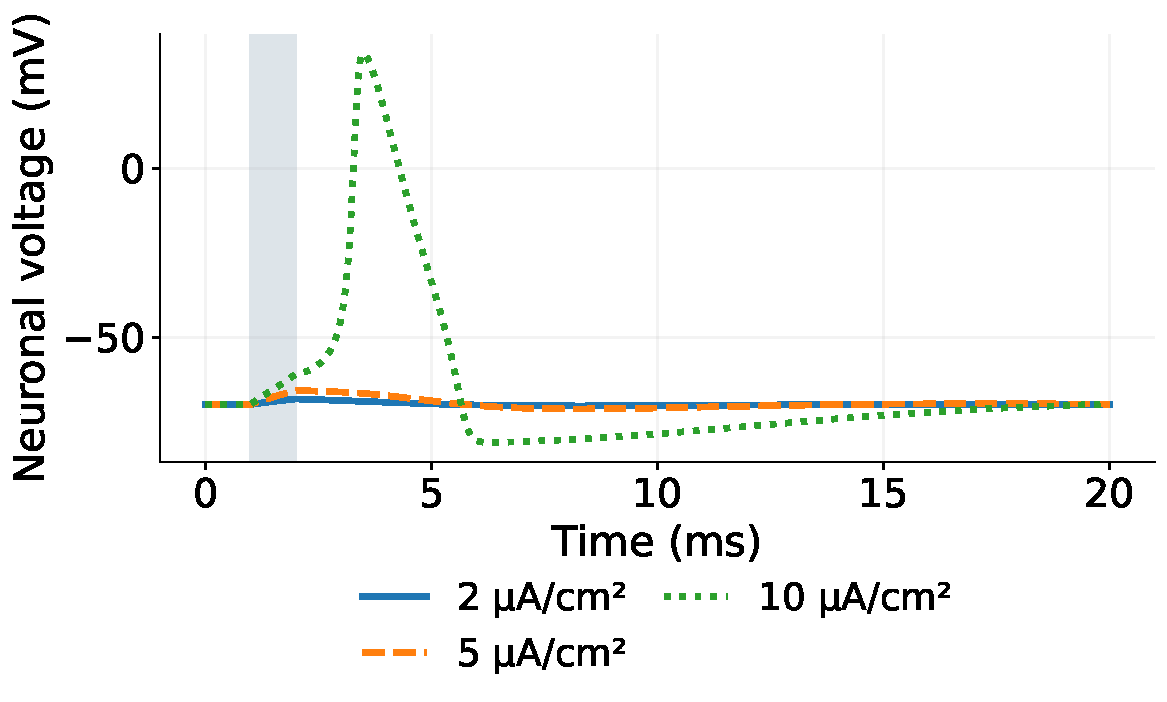
\includegraphics[width=.98\linewidth,height=.69\textheight,keepaspectratio]{presentation-figures/neuronal-cell-panel-1.pdf}\end{frame}
\renewcommand{\notestarget}{notes.pdf\#note-conductances-and-gate-relaxation}
\begin{frame}[label=slide-voltage-driving-forces-and-conductances-panel-2]{Bounded gate fractions}
\centering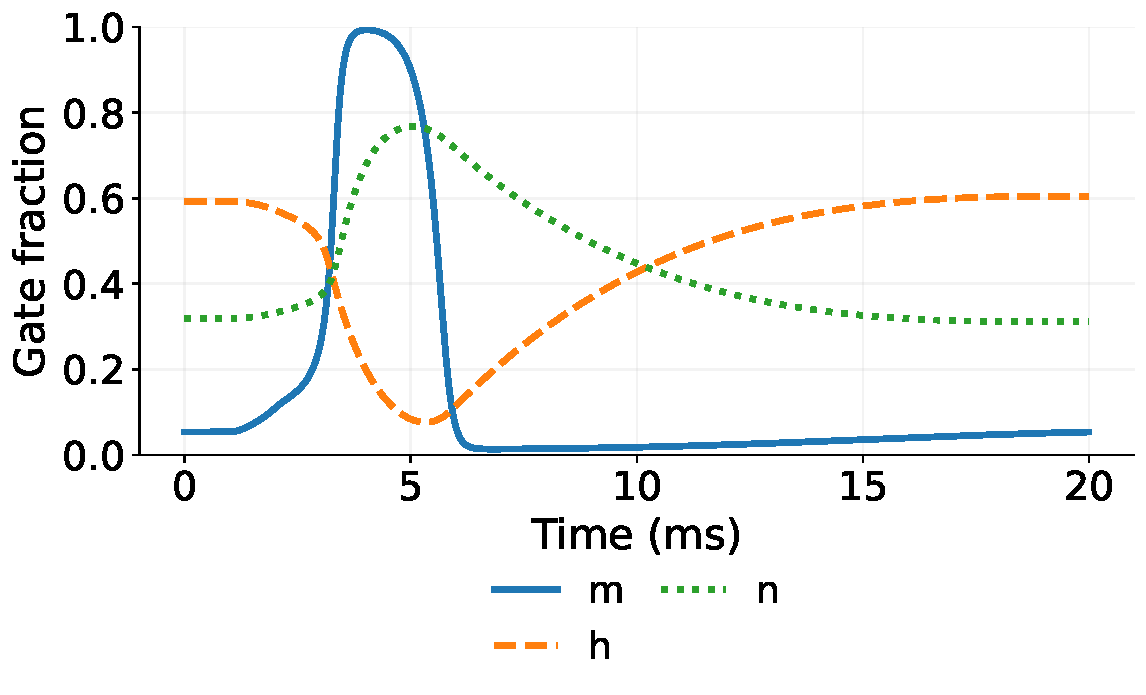
\includegraphics[width=.98\linewidth,height=.69\textheight,keepaspectratio]{presentation-figures/neuronal-cell-panel-2.pdf}\end{frame}
\renewcommand{\notestarget}{notes.pdf\#note-conductances-and-gate-relaxation}
\begin{frame}[t,fragile,label=slide-voltage-driving-forces-and-conductances]{Voltage driving forces and conductances}
\[g_{Na}=120m^3h,\qquad g_K=36n^4,\qquad g_L=.3.\]\pause{}\[(E_{Na},E_K,E_L)=(45,-82,-59)\ \mathrm{mV}.\]
\end{frame}
\renewcommand{\notestarget}{notes.pdf\#note-conductances-and-gate-relaxation}
\begin{frame}[t,fragile,label=slide-the-gate-equation]{The gate equation}
\[\dot s=\alpha_s(V)(1-s)-\beta_s(V)s.\]\pause{}\[s_\infty=\frac{\alpha_s}{\alpha_s+\beta_s},\qquad \tau_s=\frac1{\alpha_s+\beta_s}.\]
\end{frame}
\renewcommand{\notestarget}{notes.pdf\#note-conductances-and-gate-relaxation}
\begin{frame}[t,fragile,label=slide-bounds-of-the-continuous-gate]{Bounds of the continuous gate}
At $s=0$, $\dot s=\alpha_s\ge0$. At $s=1$, $\dot s=-\beta_s\le0$.\pause{} The vector field points into the admissible interval.
\end{frame}
\renewcommand{\notestarget}{notes.pdf\#note-finite-evaluation-of-the-rate-functions}
\begin{frame}[t,fragile,label=slide-the-removable-rate-singularity]{The removable rate singularity}
\[f(z)=\frac z{1-e^{-z}},\qquad f(0)=1.\]\pause{}\[f(z)=1+z/2+z^2/12-z^4/720+O(z^6).\]
\end{frame}
\renewcommand{\notestarget}{notes.pdf\#note-finite-evaluation-of-the-rate-functions}
\begin{frame}[t,fragile,label=slide-two-activation-rates]{Two activation rates}
\[\alpha_m=f((V+45)/10),\qquad\alpha_n=.1f((V+60)/10).\]\pause{} At $V=-45$ and $-60$ mV, the respective rates are $1$ and $.1\ \mathrm{ms}^{-1}$.
\end{frame}
\renewcommand{\notestarget}{notes.pdf\#note-exponential-gate-and-voltage-substeps}
\begin{frame}[t,fragile,label=slide-an-exact-frozen-voltage-gate-step]{An exact frozen-voltage gate step}
For $k_s=\alpha_s+\beta_s>0$,\[s^{n+1}=s_\infty+(s^n-s_\infty)e^{-k_s\Delta t}.\]\pause{} This is a convex combination of $s^n$ and $s_\infty$ for nonnegative rates.
\end{frame}
\renewcommand{\notestarget}{notes.pdf\#note-exponential-gate-and-voltage-substeps}
\begin{frame}[t,fragile,label=slide-the-zero-rate-limit]{The zero-rate limit}
If $\alpha_s=\beta_s=0$, then $\dot s=0$ and $s^{n+1}=s^n$.\pause{} No equilibrium fraction needs to be formed by division by zero.
\end{frame}
\renewcommand{\notestarget}{notes.pdf\#note-exponential-gate-and-voltage-substeps}
\begin{frame}[t,fragile,label=slide-freeze-conductances-after-the-gate-step]{Freeze conductances after the gate step}
\[G=\sum_jg_j,\qquad B=\sum_jg_jE_j+I.\]\pause{}\[C\dot V=B-GV,\qquad V_\infty=B/G.\]
\end{frame}
\renewcommand{\notestarget}{notes.pdf\#note-exponential-gate-and-voltage-substeps}
\begin{frame}[label=slide-an-exact-frozen-conductance-voltage-step-panel-1]{First-order coupled error}
\centering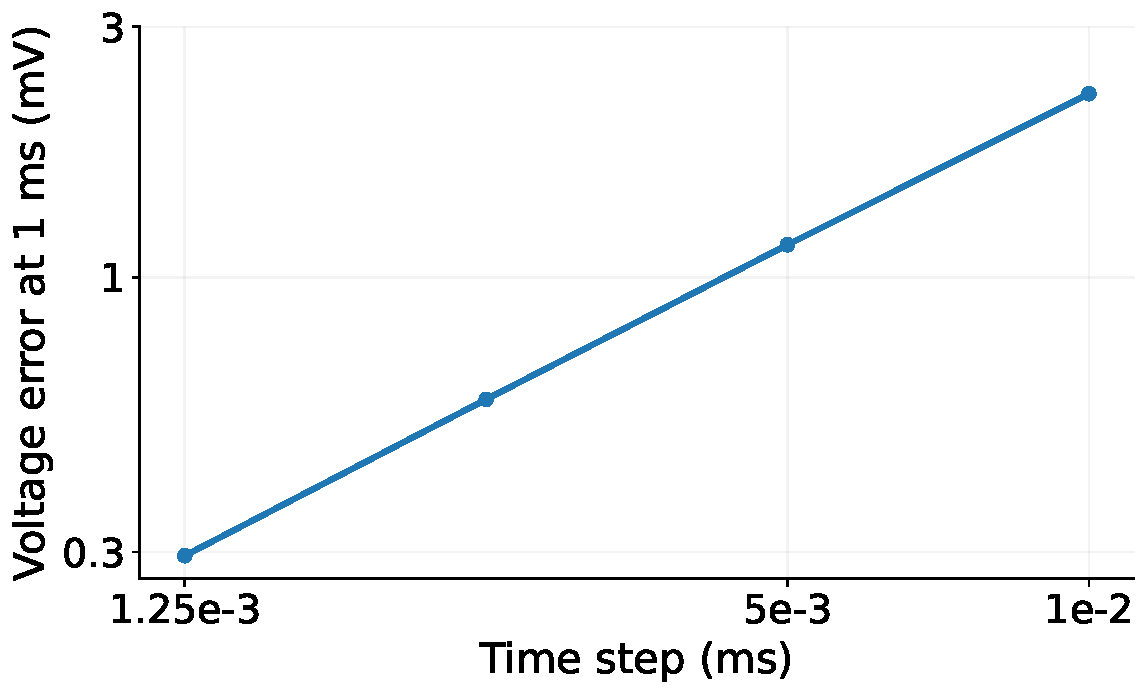
\includegraphics[width=.98\linewidth,height=.69\textheight,keepaspectratio]{presentation-figures/gate-and-time-checks-panel-1.pdf}\end{frame}
\renewcommand{\notestarget}{notes.pdf\#note-exponential-gate-and-voltage-substeps}
\begin{frame}[label=slide-an-exact-frozen-conductance-voltage-step-panel-2]{Frozen-rate gate check}
\centering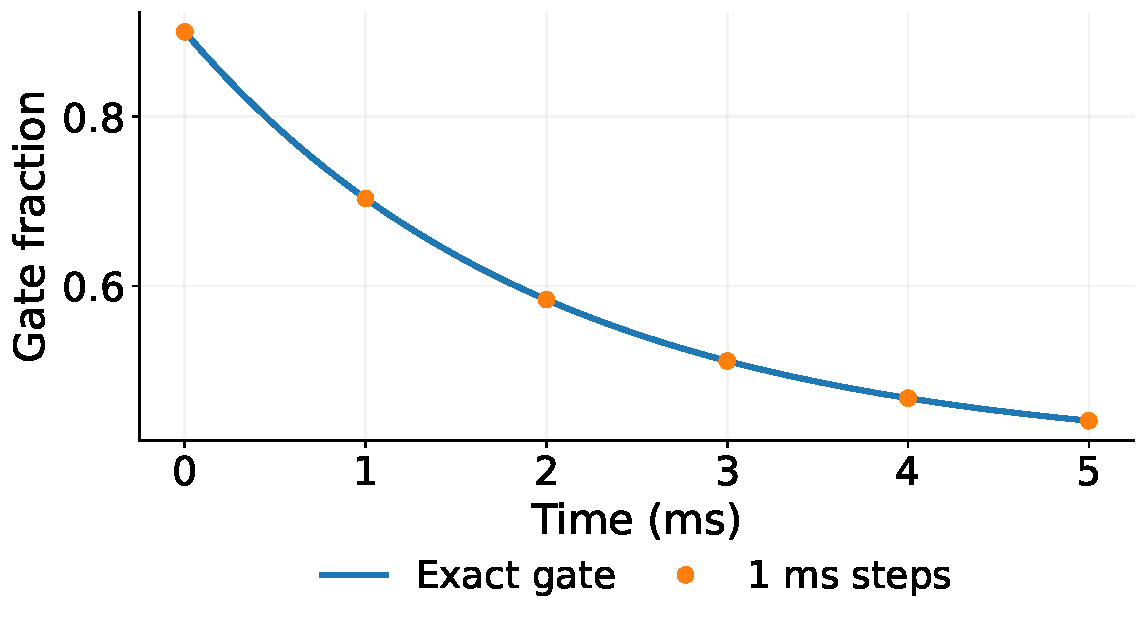
\includegraphics[width=.98\linewidth,height=.69\textheight,keepaspectratio]{presentation-figures/gate-and-time-checks-panel-2.pdf}\end{frame}
\renewcommand{\notestarget}{notes.pdf\#note-exponential-gate-and-voltage-substeps}
\begin{frame}[t,fragile,label=slide-an-exact-frozen-conductance-voltage-step]{An exact frozen-conductance voltage step}
\[V^{n+1}=V_\infty+(V^n-V_\infty)e^{-G\Delta t/C}.\]\pause{} The two exact substeps form a first-order coupled method.
\end{frame}
\renewcommand{\notestarget}{notes.pdf\#note-the-coupled-resting-state-and-stimulus-response}
\begin{frame}[t,fragile,label=slide-the-coupled-rest-equation]{The coupled rest equation}
\[\mathcal I(V)=\sum_jg_j(s_\infty(V))(V-E_j)=0.\]\pause{} Resting gates and zero net current must hold at the same voltage.
\end{frame}
\renewcommand{\notestarget}{notes.pdf\#note-the-coupled-resting-state-and-stimulus-response}
\begin{frame}[t,fragile,label=slide-current-cancellation-at-rest]{Current cancellation at rest}
Individual ionic currents can remain nonzero while their sum vanishes.\pause{} The companion recomputes the equilibrium from its exact rate constants, near $-69.89767$ mV.
\end{frame}
\renewcommand{\notestarget}{notes.pdf\#note-the-coupled-resting-state-and-stimulus-response}
\begin{frame}[t,fragile,label=slide-excitation-depends-on-the-protocol]{Excitation depends on the protocol}
Pulse amplitude, duration, initial voltage and initial gates jointly determine the response.\pause{} A zero-crossing distinction for one pulse does not define a universal excitation threshold.
\end{frame}
\renewcommand{\notestarget}{notes.pdf\#note-neuronal-and-reduced-cardiac-model-identities}
\begin{frame}[t,fragile,label=slide-model-identity]{Model identity}
These neuronal kinetics describe a specific $V,m,h,n$ system.\pause{} A reduced cardiac model changes both the variables and the equations; it is not obtained by relabeling a neuronal trace.
\end{frame}
\end{document}
